% !TEX TS-program = pdflatex
% !TEX encoding = UTF-8 Unicode

% TO COMPILE: lmake (animal scrifices may be necessary)
%%%%%%%%%%%%%%%%%%%%%%%%%%%%%%%%%%%%%%%%%%%%%%%%%%%%%%%%%%%%%%%%%%%%%%%%%%
%																							                           %
%				                         PREAMBLE      							             %
%                                                                        %
%%%%%%%%%%%%%%%%%%%%%%%%%%%%%%%%%%%%%%%%%%%%%%%%%%%%%%%%%%%%%%%%%%%%%%%%%%
\documentclass[compress]{beamer}

\mode<presentation>
{
  \usetheme{Frankfurt}
  \usecolortheme{crane}
  \setbeamercovered{transparent}
}

% Package Setup
%%%%%%%%%%%%%%%%%%%%%%%%%%%%%%%%%%%%%%%%%%%%%%%%%%%%%%%%%%%%%%%%%%%%%%%%%%
%                                                                        %
%                                 PREAMBLE                               %
%                                                                        %
%%%%%%%%%%%%%%%%%%%%%%%%%%%%%%%%%%%%%%%%%%%%%%%%%%%%%%%%%%%%%%%%%%%%%%%%%%

%% PACKAGES
\usepackage[]{lineno}
\usepackage{fancyvrb}
%\linenumbers
\usepackage{amsmath}
\usepackage{microtype}
\usepackage{algorithmic}

%% GRAPHICS RELATED
\usepackage{graphicx}
\usepackage[outdir=./tmp/]{epstopdf}
\graphicspath{{../images/}{./}{./tmp/}}
\DeclareGraphicsExtensions{.eps, .pdf, .jpeg, .png}

%% CAPTION SETUP
\usepackage{float}
\usepackage[font=footnotesize]{caption}
\usepackage[font=small]{subcaption}
\captionsetup{belowskip=12pt,aboveskip=4pt}

%% BEAMER
\usepackage{multicol}
\usepackage{multirow}
\usepackage{array}				% Table Stuff
\usepackage{arydshln}
\usepackage{rotating}

%% BIBLIOGRAPHY
\bibliographystyle{ieeetr}

%% UNITS
\usepackage{siunitx}

%% EQUATIONS
%\numberwithin{equation}{section}

%%%%%%%%%%%%%%%%%%%%%%%%%%%%%%%%%%%%%%%%%%%%%%%%%%%%%%%%%%%%%%%%%%%%%%%%%%%
%                                                                         %
%                             Listing Setup                               %
%                                                                         %
%%%%%%%%%%%%%%%%%%%%%%%%%%%%%%%%%%%%%%%%%%%%%%%%%%%%%%%%%%%%%%%%%%%%%%%%%%%
\usepackage{listings}
\lstset{ %
    language=C++,
    basicstyle=\footnotesize\ttfamily,
    numbers=left,
    numberstyle=\tiny\color{gray},
    stepnumber=2,
    numbersep=5pt,
    backgroundcolor=\color{white},
    showspaces=false,
    showstringspaces=false,
    showtabs=false,
    frame=single,
    rulecolor=\color{black},
    tabsize=2,
    breaklines=true,
    breakatwhitespace=false,
    title=\lstname,
    keywordstyle=\color{blue},
    commentstyle=\color{OliveGreen},
    stringstyle=\color{orange}
}
\DeclareCaptionFont{white}{\color{white}}
\DeclareCaptionFormat{listing}{\colorbox[cmyk]{0.43, 0.35, 0.35, 0.01}{\parbox{\dimexpr\textwidth-2\fboxsep\relax}{#1#2#3}}}
\captionsetup[lstlisting]{format=listing,labelfont=white,textfont=white,singlelinecheck=false,margin=0pt,font={bf,footnotesize}}
%\lstnewenvironment{code}[1][]%
%{ \noindent\minipage{\linewidth}
%	\lstset{#1}
%}
%{\endminipage}
%% USER COMMANDS
\usepackage{isotope}
\newcommand{\iso}{\isotope}
\newcommand{\figurewidth}{\textwidth}
\newcommand{\micron}{$\mu$m}



% Preamble / Frst Size
%\setbeamersize{text margin left=5mm, text margin right 5mm}
\title[RPM8 Optimiziation] {Optimization of the RPM8 Detector with Genetic Algorthims}
\author[] {
    Matthew Urffer\inst{1}
}
\institute[University of Tennessee] { 
  \inst{1}%
  Department of Nuclear Engineering,
  University of Tennessee, Knoxville, TN
}

\date[] {March 3, 2013}
\pgfdeclareimage[height=0.5cm]{university-logo}{../images/utwordmarkhorz.png}
\logo{\pgfuseimage{university-logo}}

\begin{document}

\begin{frame}[plain]
  \titlepage
  \tiny
    \begin{center}
\centering{Financial support from the Domestic Nuclear Detection Office (DNDO) through Award No. 003387891 is gratefully acknowledged. 
  Any opinions, findings, and conclusions or recomendations expressed in this material are those of the presenter and do not necessarily reflect the views of DNDO.}
  \end{center}
\end{frame}

\begin{frame}{Table of Contents}
  \begin{multicols}{2}
    %\tableofcontents[currentsection,pausesections]
    \tableofcontents[currentsection]
    \end{multicols}
\end{frame}


%%%%%%%%%%%%%%%%%%%%%%%%%%%%%%%%%%%%%%%%%%%%%%%%%%%%%%%%%%%%%%%%%%%%%%%%%%
%                                                                        %
%                          START OF CONTENT                              %
%                                                                        %
%%%%%%%%%%%%%%%%%%%%%%%%%%%%%%%%%%%%%%%%%%%%%%%%%%%%%%%%%%%%%%%%%%%%%%%%%%
\section{Introduction}
\begin{frame}{Introduction}
What geometry is best for the RPM8
\end{frame}
%%%%%%%%%%%%%%%%%%%%%%%%%%%%%%%%%%%%%%%%%%%%%%%%%%%%%%%%%%%%%%%%%%%%%%%%%%
\begin{frame}{Design Constraints}
\begin{itemize}
  \item Count rate 
  \item Fit inside RPM8 Footprint
\end{itemize}
\end{frame}
%%%%%%%%%%%%%%%%%%%%%%%%%%%%%%%%%%%%%%%%%%%%%%%%%%%%%%%%%%%%%%%%%%%%%%%%%%
\begin{frame}{Previous Work}
  \item Have and idea on what thickness of moderator we need
\begin{figure}
  \begin{subfigure}[b]{0.45\textwidth}
    \centering
    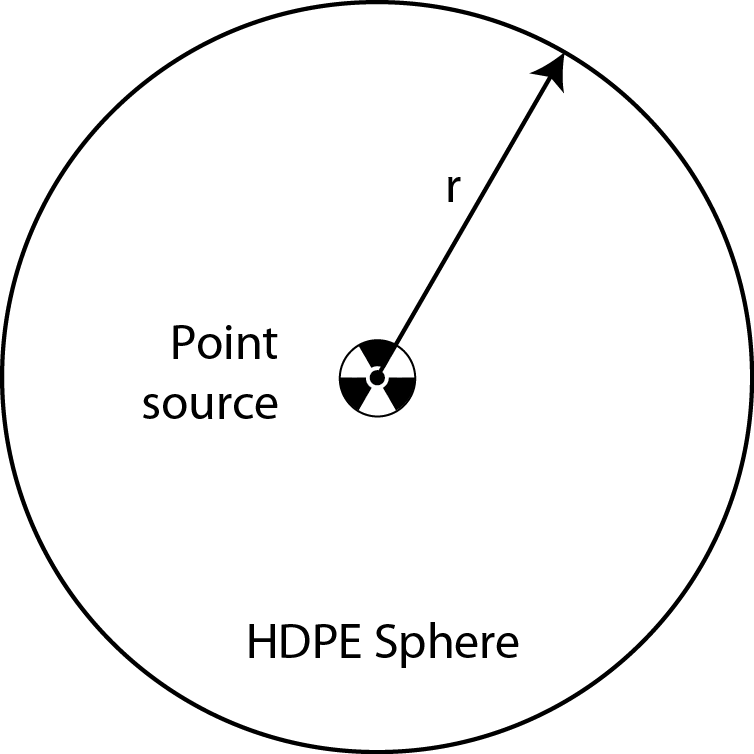
\includegraphics[width=\textwidth]{HDPEModeration_PointSrcGeo}
    \caption{Geometry of mono energetic point source}
  \end{subfigure}%
  ~
  \begin{subfigure}[b]{0.45\textwidth}
    \centering
    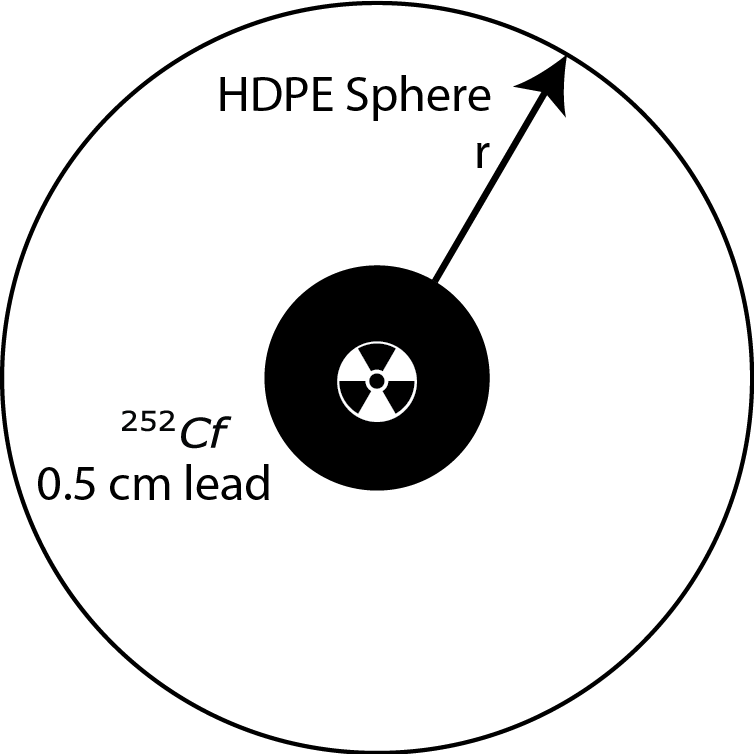
\includegraphics[width=\textwidth]{HDPEModeration_Cf252SrcGeo}
    \caption{Geometry of \isotope[252]{Cf} source}
  \end{subfigure}
  \caption{Simulated Geometry}
\end{figure}
\begin{figure}
	\centering
	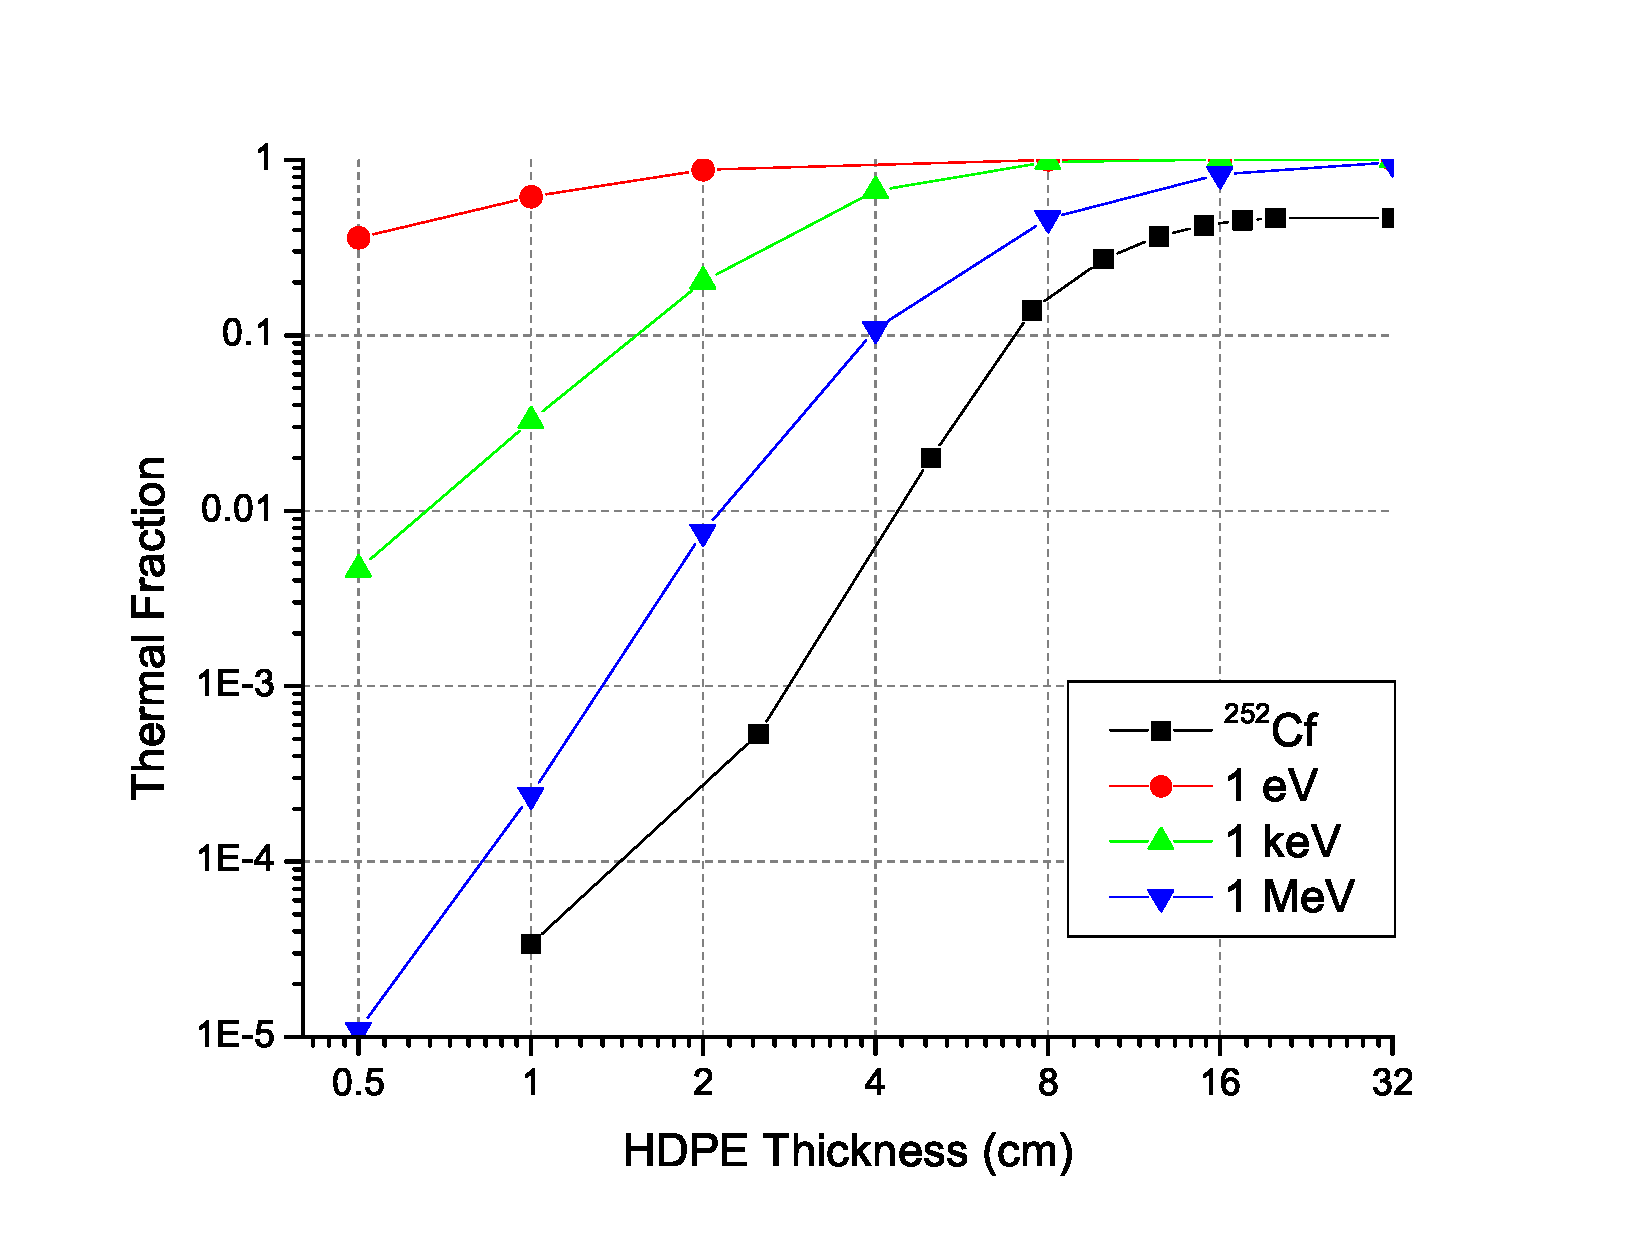
\includegraphics[width=\textwidth]{HDPEModThermalFraction}
	\caption{Thermal Neutron Fraction}
\end{figure}
\end{frame}
%%%%%%%%%%%%%%%%%%%%%%%%%%%%%%%%%%%%%%%%%%%%%%%%%%%%%%%%%%%%%%%%%%%%%%%%%%
%%%%%%%%%%%%%%%%%%%%%%%%%%%%%%%%%%%%%%%%%%%%%%%%%%%%%%%%%%%%%%%%%%%%%%%%%%
\section{Genatic Algorthims}
%% Genatic Algorthims introduction

%%%%%%%%%%%%%%%%%%%%%%%%%%%%%%%%%%%%%%%%%%%%%%%%%%%%%%%%%%%%%%%%%%%%%%%%%%
%                                                                        %
%                      Pyevole Introduction                              %
%                                                                        %
%%%%%%%%%%%%%%%%%%%%%%%%%%%%%%%%%%%%%%%%%%%%%%%%%%%%%%%%%%%%%%%%%%%%%%%%%%
\subsection{PyEvolve}
\begin{frame}{PyEvolve Introduction}
	\begin{itemize}
  \small
  \item PyEvolve is a genetic algorithm framework written in pure python
  \item Genetic Algorithm Features:
    \begin{itemize}
      \item Crossover operations (single point, two point, uniform)
      \item Mutator operations (swap, flip)
      \item Selection operations (rank, uniform, tournament, roulette)
    \end{itemize}
  \item Additional Features:
    \begin{itemize}
      \item Run statistics
      \item Convergence criteria
      \item Function callbacks
    \end{itemize}
  \end{itemize}
  \begin{figure}
    
\includegraphics[width=0.2\textwidth]{PyEvolveLogo.png}
  \end{figure}
\end{frame}
\begin{frame}{PyEvolve - Belly of the Lizard}
	Representation of the the Genetic Algorithm
  \begin{itemize}
    \item \texttt{GSimpleGA} genetic algorithm
    \item \texttt{GPopulation} - the population
    \item \texttt{Initializators} - initialization methods
    \item \texttt{Mutators} - collection of mutator methods
    \item \texttt{Crossovers} - collection of crossover methods
    \item \texttt{Selectors} - collection of selection methods
  \end{itemize}
  Representation of an individual
  \begin{itemize}
    \item Bit string representation \texttt{10010101}
    \item Defined in \texttt{G1DBinaryString.py}
		\item Other representations are available (tree, 2D list)
  \end{itemize}
\end{frame}

%\include{./RPM8MethodPresentation}
\section{Conclusions}
%%%%%%%%%%%%%%%%%%%%%%%%%%%%%%%%%%%%%%%%%%%%%%%%%%%%%%%%%%%%%%%%%%%%%%%%%%
\begin{frame}{Summary}

\begin{figure}
	\centering
  
\includegraphics[width=0.2\textwidth]{Questions.eps}
\end{figure}
\end{frame}

%%%%%%%%%%%%%%%%%%%%%%%%%%%%%%%%%%%%%%%%%%%%%%%%%%%%%%%%%%%%%%%%%%%%%%%%%%%
% BILBIOLGRAPHY
\begin{frame}[plain,allowframebreaks]
\frametitle{Works Cited}
	\tiny
  \bibliography{../Zotero}
\end{frame}

%%%%%%%%%%%%%%%%%%%%%%%%%%%%%%%%%%%%%%%%%%%%%%%%%%%%%%%%%%%%%%%%%%%%%%%%%%%
% APPENDIX

\end{document}


